\chapter{Cache Forwarding Example}
\label{chap:fpgasteel-cache-forwarding}

\section{Prerequisites}
\label{sec:fpgasteel-cache-forwarding-prerequisites}

Same toolchain, \term{SD card} and \term{Eclipse}/\term{OpenOCD} debug setup as Hello World (Chapter~\ref{chap:fpgasteel-hello-world}), plus the \term{OV7670} camera adapter board on \term{GPIO\_0} as described in I\textsuperscript{2}C Example (Section~\ref{sec:fpgasteel-i2c-prerequisites}).

\begin{warningbox}
\textbf{Hardware bug:} do not leave the camera in \term{RESET} or \term{POWER-DOWN} for extended periods.\footnotemark
\end{warningbox}
\footnotetext{See Part~\ref{part:appendices}, Section~\ref{sec:camera-adapter-reset-powerdown}.}

\section{About this project}
\label{sec:fpgasteel-cache-forwarding-about}

|cache_forwarding_example| (under |sw/cache_forwarding_example|) runs the exact same camera-to-\term{VGA} forwarding pipeline as |simple_forwarding_example|, over the same \term{FPGA} hardware, unchanged, but with the \term{CPU}'s data cache and the shared \term{L2} cache enabled. Enabling them means the frame buffers in \term{DDR} can be cached by the \term{CPU}, which is faster for the software side (|SimpleFilters::convert()|, in particular) but introduces a new problem absent from Simple Forwarding Example (Chapter~\ref{chap:fpgasteel-simple-forwarding}): the two \term{mSGDMA} cores that move frames in and out of \term{DDR} bypass the \term{ARM} cores' caches entirely, so the \term{CPU}'s cached view of a frame buffer can silently diverge from what is actually in \term{DDR}, the only copy the \term{DMA} cores ever see. Paragraph~\ref{subsec:fpgasteel-cache-mmu-architecture} explains why, and how this project resolves it.

Compared to Simple Forwarding Example (Chapter~\ref{chap:fpgasteel-simple-forwarding}), this project adds one step to startup: right after bringing up the interrupt controller, and before anything else runs, |System::enableCache()| enables the \term{L1} data cache, the \term{L2} cache, and the flat 1:1 section-based \term{MMU} mapping.

Everything else at startup, and in the main loop, is structurally the same as Simple Forwarding Example (Chapter~\ref{chap:fpgasteel-simple-forwarding}): |Camera| and |Vga| still run the same descriptor/prefetcher pipelines, and |SimpleFilters| still converts each captured frame to \term{RGB24} for display. The one loop-level difference is that frame buffers are now handled through |CacheAwareFrame|/|CacheAwareFramePool| (Paragraph~\ref{subsec:fpgasteel-cache-aware-frame}, Paragraph~\ref{subsec:fpgasteel-cache-aware-framepool}) instead of the plain |Frame|/|FramePool| from Simple Forwarding Example (Chapter~\ref{chap:fpgasteel-simple-forwarding}), so that the handoff between the \term{CPU} and each \term{DMA} master can carry an explicit cache flush or invalidate where one is needed.

The camera and \term{VGA} \term{ISR}s themselves, |Camera::onTransferComplete()| and |Vga::onTransferComplete()|, are unaltered: comparing this project's |Camera.cpp|/|Vga.cpp| against Simple Forwarding Example (Chapter~\ref{chap:fpgasteel-simple-forwarding})'s shows no logic difference at all.

\section{FPGA Hardware Involved}
\label{sec:fpgasteel-cache-forwarding-hardware}

Unchanged: see Section~\ref{sec:fpgasteel-simple-forwarding-hardware}. Both \term{mSGDMA} cores, their descriptor memories, and every other \term{IP} core listed there are exactly the same hardware used by this project (the \term{Avalon-ST}/\term{Avalon-MM} conventions are those defined in \cite{AVALON-SPEC}).

\section{Operating principles}
\label{sec:fpgasteel-cache-forwarding-operating-principles}

\subsection{ARM Cortex-A9 cache and MMU architecture}
\label{subsec:fpgasteel-cache-mmu-architecture}

\subsubsection{The cache and SCU hardware}
\label{subsubsec:fpgasteel-cache-scu-hardware}

The Cyclone V SoC \term{FPGA} integrates a built-in dual-core \term{ARM} Cortex-A9 processor. Each core is provided with two separate 32 KB caches, one for data and one for instructions, plus its own \term{MMU} and \term{NEON}/\term{FPU} media processing engine.

Moreover, the two cores share a single 512 KB \term{L2} cache (a \term{PL310} controller), holding both data and instructions for either core.

Keeping the two cores' private \term{L1} caches coherent with each other, and with the shared \term{L2} below them, is the job of the Snoop Control Unit (\term{SCU}): it arbitrates every \term{L1} line request coming from either core, keeps track of which core currently holds each line, and either forwards a fresh copy between the two caches or invalidates a stale one, so a write performed on one core is never left stale in the other core's cache. The \term{SCU} also hosts the global exclusive monitor used by atomic (load-exclusive/store-exclusive) instructions, which is why enabling it matters even when only one core is actually running. The \term{GIC}, a global timer, and an Accelerator Coherency Port are also shared between the two cores, alongside the \term{L2} controller.

This project (unlike |dualcore_forwarding_example|) only runs on one core, so the \term{SCU}'s role here is narrower than in a true dual-core configuration; it must still be enabled, though, since the \term{L2} controller and the cache-maintenance operations this project relies on depend on it being on (Subparagraph~\ref{subsubsec:fpgasteel-enabling-mmu}).

\begin{figure}[htbp]
    \centering
    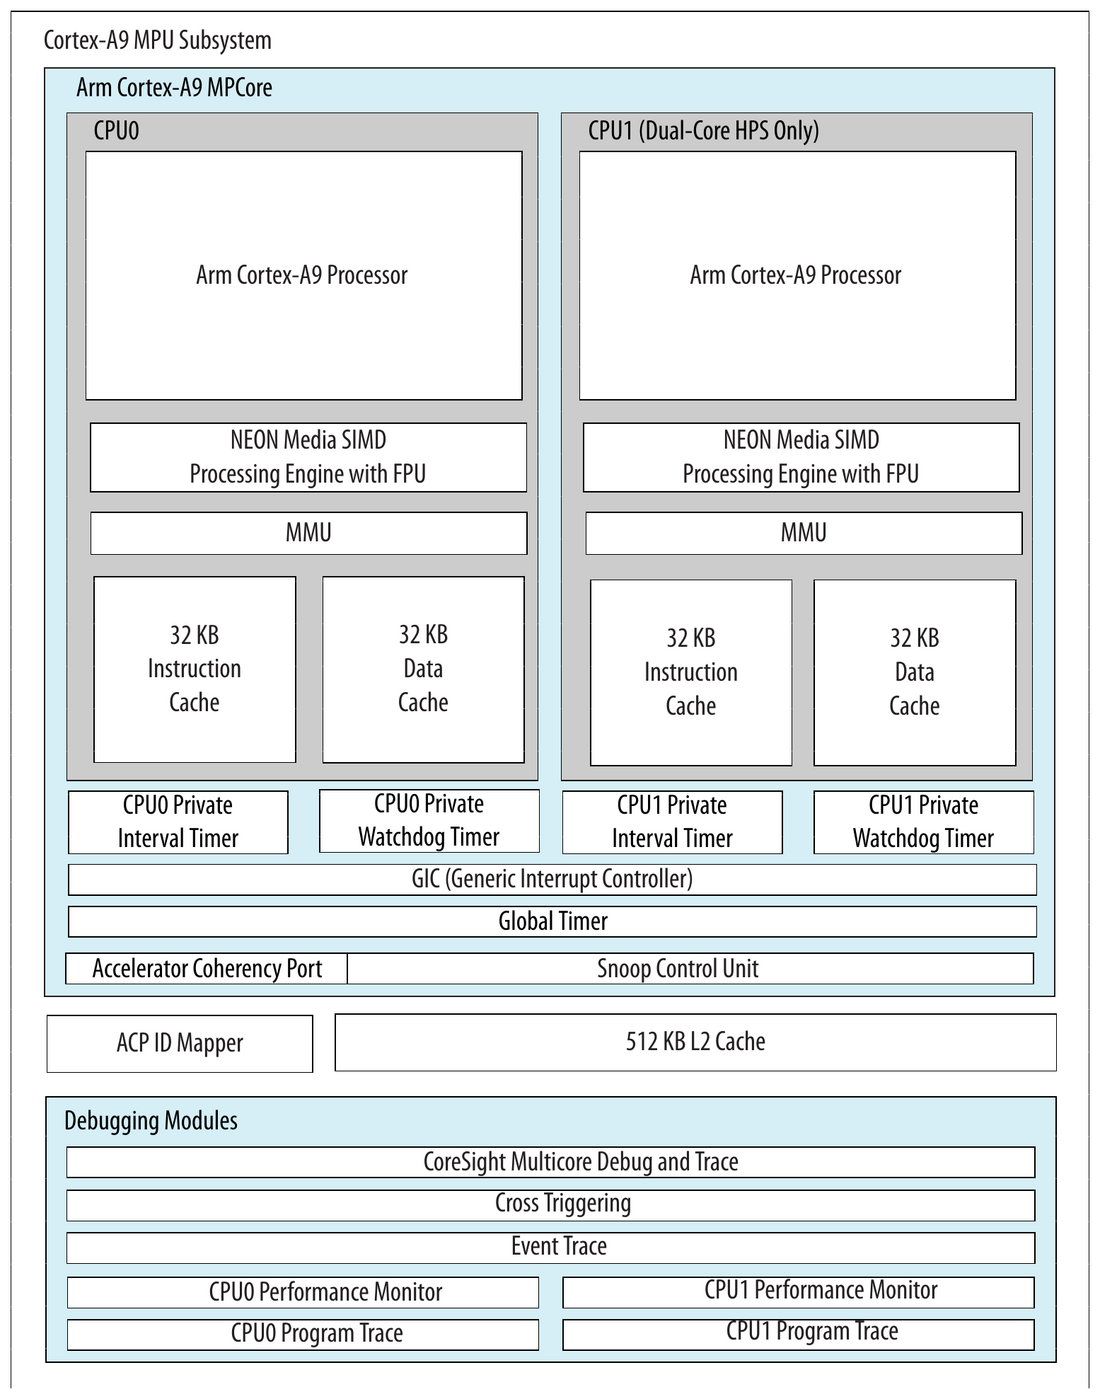
\includegraphics[width=0.9\linewidth]{img/FPGAsteelHpsTrm.png}
    \caption[Cortex-A9 MPU Subsystem Block Diagram]{Cortex-A9 MPU Subsystem Block Diagram, reproduced from \cite[Figure 10-2, p.~176]{CV-TRM}. Reported here for reference; not original work.}
    \label{fig:fpgasteel-cortex-a9-mpu-subsystem}
\end{figure}

\subsubsection{DMA vs.\ cache coherency}
\label{subsubsec:fpgasteel-dma-cache-coherency}

|Camera| and |Vga| (Paragraph~\ref{subsec:fpgasteel-cache-camera-class}, Paragraph~\ref{subsec:fpgasteel-cache-vga-class}) move frame data in and out of \term{DDR} through two \term{FPGA}-fabric \term{mSGDMA} cores. Those cores read and write \term{DDR} directly; they do not pass through the \term{ARM} cores' \term{L1}/\term{L2} cache hierarchy, and cannot snoop it. With caching enabled, this creates two distinct coherency problems, one per direction:

\begin{enumerate}
    \item \textbf{\term{CPU} writes, \term{DMA} reads.} After |SimpleFilters::convert()| writes a converted \term{RGB24} frame, that data may still sit only in the \term{CPU}'s caches, not yet written back to \term{DDR}. If |Vga|'s \term{mSGDMA} core is then pointed at that buffer, it reads stale bytes straight out of \term{DDR}, missing the \term{CPU}'s most recent writes.
    \item \textbf{\term{DMA} writes, \term{CPU} reads.} After |Camera|'s \term{mSGDMA} core writes a captured frame into a buffer, the \term{CPU} may still be holding an older copy of that same memory in cache from a previous read. If the \term{CPU} reads that buffer again without first discarding the stale copy, it sees old pixel data instead of what the \term{DMA} core just wrote.
\end{enumerate}

The fix is the same operation in both cases, just named differently depending on direction: before the \term{DMA} core reads \term{CPU}-written data, the corresponding cache lines must be cleaned (written back to \term{DDR}, also called flushing); before the \term{CPU} reads \term{DMA}-written data, the corresponding cache lines must be invalidated (discarded, so the next read is forced to fetch straight from \term{DDR}). Paragraph~\ref{subsec:fpgasteel-cache-aware-frame} covers the two methods that do this, |CacheAwareFrame::cacheFlush()| and |CacheAwareFrame::cacheInvalidate()|; Section~\ref{sec:fpgasteel-cache-forwarding-how-it-works} shows exactly where each one is called.

\subsubsection{Enabling the MMU}
\label{subsubsec:fpgasteel-enabling-mmu}

The Cortex-A9 \term{L1} data cache cannot be turned on without the \term{MMU} also being on: cacheability and shareability are per-region attributes carried by the \term{MMU}'s translation tables, not a separate switch, so the cache literally has nowhere to read those attributes from until address translation is active. This project uses the simplest translation table that satisfies that requirement: a flat 1:1 mapping (every virtual address maps to the identical physical address), declared as three regions and handed to |alt_mmu_va_space_create()| (\unresolved{\texttt{HWLib}}), which builds the actual hardware descriptors transparently, choosing whatever granularity each region's alignment and size allow. The project itself never deals with that choice:

\begin{table}[htbp]
    \centering
    \begin{tabular}{@{}l l l l l p{4.5cm}@{}}
        \hline
        \textbf{Base address} & \textbf{Size} & \textbf{Attribute} & \textbf{Shareable} & \textbf{Execute} & \textbf{Contents} \\
        \hline
        0x00000000 & 1024 MB & Cacheable, write-back write-allocate & Shareable & Enabled & \term{DDR}: code, stack, heap, frame buffers \\
        0xC0000000 & 960 MB & Non-cacheable & Non-shareable & Never (\term{XN}) & \term{HPS}-\term{FPGA} bridge: \term{mSGDMA} descriptor memories, \term{Avalon-MM} peripherals \\
        0xFC000000 & 64 MB & Device & Non-shareable & Never (\term{XN}) & \term{HPS} peripherals (\term{UART}, \term{GIC}, timers, \ldots) \\
        \hline
    \end{tabular}
    \caption[MMU section mapping built by System::enableCache()]{\term{MMU} section mapping built by System::enableCache().}
    \label{tab:fpgasteel-mmu-section-mapping}
\end{table}

The \term{DDR} region is the only one marked cacheable; the other two are left non-cacheable/device on purpose, since caching either register accesses or the descriptor memory the prefetcher polls would make software see stale values there too.

\subsubsection{HWLib performs the work}
\label{subsubsec:fpgasteel-hwlib-performs-work}

None of the above (\term{SCU}/cache/\term{MMU} manipulation) is done through custom register-level code written for this project, with one narrow exception: enabling the \term{SCU} and setting the \term{ACTLR.SMP} bit, done directly through the Arm's \term{CP15} coprocessor, since \unresolved{\term{HWLib}} has no wrapper for that specific step. Everything else, building the section table, switching the \term{MMU} on, enabling the \term{L1} data cache and the \term{L2} controller, and later cleaning or invalidating a buffer's cache lines, goes through Altera/Intel's \unresolved{\term{HWLib}} (|intel-socfpga-hwlib|):

|alt_mmu_va_space_create()|/|alt_mmu_va_space_enable()|, |alt_cache_l1_data_enable()|, |alt_cache_l2_init()|/|alt_cache_l2_enable()|, and later |alt_cache_system_clean()|/|alt_cache_system_invalidate()|. Paragraph~\ref{subsec:fpgasteel-cache-system-class} walks through |System::enableCache()|, which is where all of these calls are made, in the order they must run.

\subsection{Descriptors and the prefetcher}
\label{subsec:fpgasteel-cache-descriptors-prefetcher}

Unchanged: see Section~\ref{subsec:fpgasteel-descriptors-prefetcher}. Everything there, the descriptor layout, the ping-pong loop between |desc0|/|desc1|, |OWNED_BY_HW|, and the prefetcher itself, applies here without modification.

\subsection{Camera capture internals}
\label{subsec:fpgasteel-cache-camera-capture}

Unchanged: see Section~\ref{subsec:fpgasteel-camera-capture-interrupt}. |Camera::onTransferComplete()| runs the identical sequence; the only new step it now demands from its caller is the explicit |cacheInvalidate()| on the buffer it hands over, since the \term{ISR} itself has no reason to do that on the \term{DMA} core's behalf.

\subsection{VGA output internals}
\label{subsec:fpgasteel-cache-vga-output}

Unchanged: see Section~\ref{subsec:fpgasteel-vga-output-interrupt}. |Vga::onTransferComplete()| runs the identical sequence; the new step it now demands from its caller is the explicit |cacheFlush()| before a frame is pushed into |vgaPool|.

\section{Code structure}
\label{sec:fpgasteel-cache-code-structure}

Only the classes that differ from Simple Forwarding Example (Chapter~\ref{chap:fpgasteel-simple-forwarding}) are documented in full here; everything else is covered by reference. Paragraphs~\ref{subsec:fpgasteel-cache-system-class}--\ref{subsec:fpgasteel-cache-aware-framepool} are entirely new in this project.

\subsection{Frame class}
\label{subsec:fpgasteel-cache-frame-class}

Unchanged, with one access-level change: |m_buffer| moved from private to protected, so that |CacheAwareFrame| can reach the raw pointer directly instead of going through |getBuffer()|. No behavioral change.

\subsection{FramePool class}
\label{subsec:fpgasteel-cache-framepool}

Unchanged, with two internal changes needed to support |CacheAwareFramePool|: |MAX_SLOTS| and the |m_frameStorage| bookkeeping array moved from private to protected, and |m_queueCount| changed from a plain |volatile unsigned| to |std::atomic<unsigned>|. Neither changes the public producer/consumer \term{API} (|borrow()|/|push()|/|pop()|/|giveBack()|) or its behavior.

\subsection{PrefetcherExtendedDescriptor class}
\label{subsec:fpgasteel-cache-prefetcher-extended-descriptor}

Unchanged: see Section~\ref{subsec:fpgasteel-prefetcher-extended-descriptor}.

\subsection{MsgdmaPrefetcherMemory class}
\label{subsec:fpgasteel-cache-msgdma-prefetcher-memory}

Unchanged: see Section~\ref{subsec:fpgasteel-msgdma-prefetcher-memory}. Descriptor memory is left non-cacheable by the \term{MMU} mapping (Subparagraph~\ref{subsubsec:fpgasteel-enabling-mmu}), so this class needs no cache maintenance of its own.

\subsection{PrefetchedMSGDMA class}
\label{subsec:fpgasteel-cache-prefetched-msgdma}

Unchanged: see Section~\ref{subsec:fpgasteel-prefetched-msgdma}.

\subsection{Camera class}
\label{subsec:fpgasteel-cache-camera-class}

Unchanged: see Section~\ref{subsec:fpgasteel-camera-class}. |onTransferComplete()| is functionally identical to Simple Forwarding Example (Section~\ref{sec:fpgasteel-cache-forwarding-about} above).

\subsection{Vga class}
\label{subsec:fpgasteel-cache-vga-class}

Unchanged: see Section~\ref{subsec:fpgasteel-vga-class}. |onTransferComplete()| is functionally identical to Simple Forwarding Example.

\subsection{SimpleFilters class}
\label{subsec:fpgasteel-cache-simple-filters}

Unchanged: see Section~\ref{subsec:fpgasteel-simple-filters}.

\subsection{HexDisplay class}
\label{subsec:fpgasteel-cache-hex-display}

Unchanged: see Section~\ref{subsec:fpgasteel-hex-display}.

\subsection{System class}
\label{subsec:fpgasteel-cache-system-class}

|System| is the same singleton used in Simple Forwarding Example (Chapter~\ref{chap:fpgasteel-simple-forwarding}) (|init()|, |micros()|, |millis()|, |delay()|, |delayMicroseconds()|, |deInit()|, all identical), plus one new method this project actually relies on: |enableCache()|. Source: |src/System.{h,cpp}|.

\begin{itemize}
    \item |enableCache()|: enables the \term{L1} data cache, the \term{L2} cache, and the flat 1:1 \term{MMU} mapping discussed in Paragraph~\ref{subsec:fpgasteel-cache-mmu-architecture}. Must be called after |init()|. It performs the following actions in order:
    \begin{itemize}
        \item Enables the \term{SCU} (invalidates its tag \term{RAM}, sets its enable bit) and sets the \term{ACTLR.SMP} bit, both through direct \term{CP15} coprocessor access, since U-Boot's own startup code leaves the \term{SCU} disabled and clears \term{ACTLR}.
        \item Calls |alt_cache_system_disable()|, leaving both caches in a known, clean state before the \term{MMU} configuration underneath them changes.
        \item Builds the three-region section table from Subparagraph~\ref{subsubsec:fpgasteel-enabling-mmu} and activates it, via |alt_mmu_va_space_create()| followed by |alt_mmu_va_space_enable()|.
        \item Enables the \term{L1} data cache (|alt_cache_l1_data_enable()|) and the \term{L2} cache (|alt_cache_l2_init()| then |alt_cache_l2_enable()|).
    \end{itemize}
    Throws |ExceptionSystem| if any of the underlying |alt_mmu_*|/|alt_cache_*| calls fails.
\end{itemize}

\subsection{CacheAwareFrame class}
\label{subsec:fpgasteel-cache-aware-frame}

|CacheAwareFrame| extends |Frame| with the two cache operations Subparagraph~\ref{subsubsec:fpgasteel-dma-cache-coherency} requires, plus cache-line-aligned allocation, needed because a flush or invalidate operates on whole cache lines: performing one on a buffer that shares a line with unrelated data would flush or invalidate that neighboring data too. Source: |src/CacheAwareFrame.{h,cpp}|.

\begin{itemize}
    \item |CacheAwareFrame(width, height, colorScheme)| (overloaded constructor, form 1): allocates a new buffer via |memalign()|, aligned to |ALT_CACHE_LINE_SIZE|, owned by this object and released by the destructor. Throws |ExceptionFrame| if the allocation fails.
    \item |CacheAwareFrame(buffer, bufferSize, width, height, colorScheme)| (overloaded constructor, form 2): wraps an existing buffer, exactly like |Frame|'s equivalent constructor; the caller is responsible for making sure that buffer is itself cache-line aligned.
    \item |~CacheAwareFrame()| (destructor): frees the buffer, but only if it was allocated by form 1 above.
    \item |cacheFlush()|: cleans this frame's buffer from the \term{CPU} caches to \term{DDR} (|alt_cache_system_clean()|). Call this after the \term{CPU} has written the buffer and before a \term{DMA} master reads it.
    \item |cacheInvalidate()|: invalidates this frame's buffer in the \term{CPU} caches (|alt_cache_system_invalidate()|). Call this after a \term{DMA} master has written the buffer and before the \term{CPU} reads it.
\end{itemize}

\subsection{CacheAwareFramePool class}
\label{subsec:fpgasteel-cache-aware-framepool}

|CacheAwareFramePool| extends |FramePool| with the same two operations, applied automatically at the point where a frame changes hands between producer and consumer, so that calling code cannot forget to call them. Source: |src/CacheAwareFramePool.{h,cpp}|.

\begin{itemize}
    \item |CacheAwareFramePool(count, width, height, colorScheme)| (overloaded constructor, form 1): allocates its own cache-line-aligned storage block internally, sized |count| times a per-frame stride rounded up to a multiple of |ALT_CACHE_LINE_SIZE| (needed whenever the raw frame size is not already a multiple of the cache line size, so that one frame's buffer never shares a cache line with the next frame's). Freed by the destructor.
    \item |CacheAwareFramePool(count, width, height, colorScheme, storage)| (overloaded constructor, form 2): uses caller-provided storage instead. Throws |ExceptionFramePool| if |storage| is not itself cache-line aligned.
    \item |~CacheAwareFramePool()| (destructor): frees the storage block, but only if it was allocated by form 1 above.
    \item |push(frame, flushCache)|: if |flushCache| is true, calls |frame->cacheFlush()| first, then forwards to |FramePool::push()|.
    \item |pop(invalidateCache)|: forwards to |FramePool::pop()|; if |invalidateCache| is true, calls |cacheInvalidate()| on the returned frame before returning it.
\end{itemize}

\section{How it works}
\label{sec:fpgasteel-cache-forwarding-how-it-works}

The following snippet is taken from |main.cpp|:

\begin{lstlisting}[language=C++]
System::getInstance().init();
sys->enableCache();
// L1 D-cache + L2 + flat 1:1 MMU (Section 8.5.10)
Serial::getInstance().init();
CacheAwareFramePool camPool(CAMERA_POOL_SIZE, FRAME_WIDTH, FRAME_HEIGHT, CAMERA_COLOR_SCHEME);
CacheAwareFramePool vgaPool(VGA_POOL_SIZE, FRAME_WIDTH, FRAME_HEIGHT, Frame::ColorScheme::RGB24);
vga->init(vgaPool);
pclkResetCtrl->deassertReset();
sys->delay(1000); // test pattern shows immediately
// release the camera from reset
camera->init(camPool);
camera->verticalFlip(true);
camera->horizontalMirror(true); // configure OV7670, start ST->MM capture
hex->showDashes();
while (true) {
    // ISR fault checks omitted here, see Camera::hasIsrFault()/Vga::hasIsrFault()
    if (camPool.available() > 0) {
        CacheAwareFrame * camFrame = camPool.pop(true);
        // invalidate: DMA wrote, CPU will read
        CacheAwareFrame * vgaFrame = static_cast<CacheAwareFrame *>(vgaPool.borrow());
        uint64_t t0 = sys->millis();
        SimpleFilters::convert(*camFrame, *vgaFrame);
        uint64_t t1 = sys->millis();
        camPool.giveBack(camFrame);
        vgaPool.push(vgaFrame, true);
        // RGB565 -> RGB24
        // flush: CPU wrote, DMA will read
        hex->showNumber(static_cast<uint32_t>(t1 - t0));
    }
}
\end{lstlisting}

Each cache call above fires at the exact moment a buffer changes hands between the \term{CPU} and a \term{DMA} master, matching one of the two directions from Subparagraph~\ref{subsubsec:fpgasteel-dma-cache-coherency}:

\begin{itemize}
    \item |camPool.pop(true)| handles the ``\term{DMA} writes, \term{CPU} reads'' case: |Camera|'s \term{mSGDMA} core has just written a captured frame into \term{DDR}, and the \term{CPU} is about to use it inside |SimpleFilters::convert()|. Invalidating the cache first forces a read out to \term{DDR}, so it actually sees what the \term{DMA} core wrote.
    \item |vgaPool.push(vgaFrame, true)| handles the ``\term{CPU} writes, \term{DMA} reads'' case: |SimpleFilters::convert()| has just written a converted \term{RGB24} frame on the \term{CPU}, and |Vga|'s \term{mSGDMA} core is about to read it. Flushing first pushes those \term{CPU} writes out to \term{DDR}, so the \term{DMA} core doesn't read a buffer that is only partially, or not yet, written back.
\end{itemize}

Neither |borrow()| nor |giveBack()| needs a cache operation of its own: both only touch bookkeeping state inside |FramePool|, never the pixel buffer itself.

\section{Debug tooling}
\label{sec:fpgasteel-cache-forwarding-debug-tooling}

|debugTools/view_frame.py|, same tool as in Simple Forwarding Example (Chapter~\ref{chap:fpgasteel-simple-forwarding}), works unchanged here. One caveat specific to this project: a raw memory dump (e.g.\ via \term{GDB} |dump memory|) reads \term{DDR} directly, not through the \term{CPU}'s caches, so a buffer whose cache lines have not been flushed yet may still show stale data in the dump. When inspecting a \term{CPU}-written buffer with this tool, dump it after the corresponding |cacheFlush()|, i.e.\ after |push(frame, true)| has run.

\section{References}
\label{sec:fpgasteel-cache-forwarding-references}

\begin{itemize}
    \item \unresolved{\textbf{HWLib headers} (\texttt{alt\_cache.h}, \texttt{alt\_mmu.h}), from \texttt{intel-socfpga-hwlib}. Cache/\term{MMU} function reference behind \texttt{System::enableCache()} (used in Paragraph~\ref{subsec:fpgasteel-cache-system-class}) and \texttt{CacheAwareFrame}/\texttt{CacheAwareFramePool} (used in Paragraph~\ref{subsec:fpgasteel-cache-aware-frame}, used in Paragraph~\ref{subsec:fpgasteel-cache-aware-framepool}).}
    \item \unresolved{\textbf{Quartus 22.1 HAL headers} (\texttt{altera\_msgdma\_csr\_regs.h}, \texttt{altera\_msgdma\_prefetcher\_regs.h}, \texttt{altera\_msgdma\_descriptor\_regs.h}, \texttt{altera\_msgdma\_response\_regs.h}). Register/bit definitions behind \texttt{PrefetchedMSGDMA} and \texttt{PrefetcherExtendedDescriptor}.}
\end{itemize}
